\documentclass[14pt,a4paper]{extarticle}
% =============================================================
% preamble.tex — оформление отчётов по СТП БГУИР 01-2024
% =============================================================

% Шрифты: под pdflatex — Times через tempora + T2A,
% под xelatex/tectonic — системный Times New Roman (запасной вариант STIX Two Text)
\usepackage{iftex}
\ifPDFTeX
  \usepackage[utf8]{inputenc}
  \usepackage[T2A]{fontenc}
  \usepackage{tempora}
\else
  \usepackage{fontspec}
  \IfFontExistsTF{Times New Roman}
    {\setmainfont{Times New Roman}}
    {\setmainfont{STIX Two Text}}
  \IfFontExistsTF{DejaVu Sans Mono}
    {\setmonofont{DejaVu Sans Mono}[Scale=0.82]}
    {\setmonofont{DejaVuSansMono}[Extension=.ttf, BoldFont=*-Bold,
                                  ItalicFont=*-Oblique, Scale=0.82]}
\fi
\usepackage[russian]{babel}

% Поля: слева 30 мм, справа 15 мм, сверху и снизу 20 мм
\usepackage{geometry}
\geometry{left=30mm, right=15mm, top=20mm, bottom=20mm}

\usepackage{setspace}
\singlespacing

\pretolerance=1000
\tolerance=2000
\emergencystretch=3em

\usepackage{indentfirst}
\setlength{\parindent}{1.25cm}

% Номер страницы — снизу справа
\usepackage{fancyhdr}
\pagestyle{fancy}
\fancyhf{}
\fancyfoot[R]{\thepage}
\renewcommand{\headrulewidth}{0pt}
\fancypagestyle{plain}{%
  \fancyhf{}%
  \fancyfoot[R]{\thepage}%
  \renewcommand{\headrulewidth}{0pt}%
}

\usepackage{amsmath,amssymb}
\usepackage{graphicx}
\usepackage{float}
\usepackage{booktabs}
\usepackage{tabularx}
\usepackage{multirow}
\usepackage{longtable}
\usepackage{array}

\usepackage{caption}
\captionsetup[figure]{labelsep=endash, justification=centering,
                      font={normalsize}, name=Рисунок}
\captionsetup[table]{labelsep=endash, justification=raggedright,
                     singlelinecheck=false, font={normalsize}, name=Таблица}

\usepackage{titlesec}
\titleformat{\section}
  {\normalfont\fontsize{14}{18}\selectfont\bfseries}
  {\thesection}{0.5em}{\MakeUppercase}
\titlespacing*{\section}{1.25cm}{0pt}{14pt}
% Разрыв страницы до заголовка, чтобы номер в содержании совпадал со страницей раздела
\newcommand{\sectionbreak}{\clearpage}
\titleformat{\subsection}
  {\normalfont\fontsize{14}{18}\selectfont\bfseries}
  {\thesubsection}{0.5em}{}
\titlespacing*{\subsection}{1.25cm}{14pt}{14pt}
\titleformat{\subsubsection}
  {\normalfont\fontsize{14}{18}\selectfont\bfseries}
  {\thesubsubsection}{0.5em}{}
\titlespacing*{\subsubsection}{1.25cm}{14pt}{14pt}

\newcommand{\sectioncenter}[1]{%
  \newpage
  \phantomsection
  \addcontentsline{toc}{section}{#1}
  \begin{center}\textbf{\MakeUppercase{#1}}\end{center}
  \vspace{14pt}
}

\usepackage{tocloft}
\renewcommand{\cftsecfont}{\normalfont}
\renewcommand{\cftsecpagefont}{\normalfont}
\renewcommand{\cftsubsecfont}{\normalfont}
\renewcommand{\cftsubsecpagefont}{\normalfont}
\renewcommand{\cftsecleader}{\cftdotfill{\cftdotsep}}
\renewcommand{\cftdotsep}{1}
% babel переопределяет заголовки после преамбулы, поэтому правим через \addto
\addto\captionsrussian{\renewcommand{\contentsname}{\hfill\textbf{СОДЕРЖАНИЕ}\hfill}}
\renewcommand{\cftaftertoctitle}{\hfill}

\usepackage{enumitem}
\setlist[itemize]{noitemsep, topsep=0pt, leftmargin=1.25cm, label=--}
\setlist[enumerate]{noitemsep, topsep=0pt, leftmargin=1.25cm}

% Листинги кода и вывода программы
\usepackage{listings}
\usepackage{fancyvrb}
\lstset{
  basicstyle=\ttfamily\footnotesize,
  frame=single,
  breaklines=true,
  showstringspaces=false,
  inputencoding=utf8,
  extendedchars=true,
  columns=fullflexible,
  keepspaces=true,
  captionpos=t
}
\ifPDFTeX
\lstset{
  literate={а}{{\cyra}}1 {б}{{\cyrb}}1 {в}{{\cyrv}}1 {г}{{\cyrg}}1
           {д}{{\cyrd}}1 {е}{{\cyre}}1 {ж}{{\cyrzh}}1 {з}{{\cyrz}}1
           {и}{{\cyri}}1 {й}{{\cyrishrt}}1 {к}{{\cyrk}}1 {л}{{\cyrl}}1
           {м}{{\cyrm}}1 {н}{{\cyrn}}1 {о}{{\cyro}}1 {п}{{\cyrp}}1
           {р}{{\cyrr}}1 {с}{{\cyrs}}1 {т}{{\cyrt}}1 {у}{{\cyru}}1
           {ф}{{\cyrf}}1 {х}{{\cyrh}}1 {ц}{{\cyrc}}1 {ч}{{\cyrch}}1
           {ш}{{\cyrsh}}1 {щ}{{\cyrshch}}1 {ъ}{{\cyrhrdsn}}1
           {ы}{{\cyrery}}1 {ь}{{\cyrsftsn}}1 {э}{{\cyrerev}}1
           {ю}{{\cyryu}}1 {я}{{\cyrya}}1 {ё}{{\cyryo}}1
           {А}{{\CYRA}}1 {Б}{{\CYRB}}1 {В}{{\CYRV}}1 {Г}{{\CYRG}}1
           {Д}{{\CYRD}}1 {Е}{{\CYRE}}1 {Ж}{{\CYRZH}}1 {З}{{\CYRZ}}1
           {И}{{\CYRI}}1 {Й}{{\CYRISHRT}}1 {К}{{\CYRK}}1 {Л}{{\CYRL}}1
           {М}{{\CYRM}}1 {Н}{{\CYRN}}1 {О}{{\CYRO}}1 {П}{{\CYRP}}1
           {Р}{{\CYRR}}1 {С}{{\CYRS}}1 {Т}{{\CYRT}}1 {У}{{\CYRU}}1
           {Ф}{{\CYRF}}1 {Х}{{\CYRH}}1 {Ц}{{\CYRC}}1 {Ч}{{\CYRCH}}1
           {Ш}{{\CYRSH}}1 {Щ}{{\CYRSHCH}}1 {Ъ}{{\CYRHRDSN}}1
           {Ы}{{\CYRERY}}1 {Ь}{{\CYRSFTSN}}1 {Э}{{\CYREREV}}1
           {Ю}{{\CYRYU}}1 {Я}{{\CYRYA}}1 {Ё}{{\CYRYO}}1
           {—}{{---}}1 {–}{{--}}1 {…}{{\ldots}}1
}
\fi

% Подписи листингов — в том же стиле, что таблицы: «Листинг X.Y — Название»
\captionsetup[lstlisting]{labelsep=endash, justification=raggedright,
                          singlelinecheck=false, font={normalsize}}
\renewcommand{\lstlistingname}{Листинг}
\AtBeginDocument{\numberwithin{lstlisting}{section}}

\lstdefinestyle{python}{language=Python, keywordstyle=\bfseries}
\lstdefinestyle{shell}{language=bash, keywordstyle=\mdseries}
\lstdefinestyle{plain}{language={}, basicstyle=\ttfamily\scriptsize}

% Абзац после листинга должен сохранять отступ 1,25 см (СТП 2.1.1)
\makeatletter
\AtBeginDocument{\let\@endpetrue\@endpefalse}
\makeatother

% Подпись к блоку verbatim: \captionof вне плавающего окружения
% глобально обнуляет \parindent, поэтому отступ восстанавливается вручную
\newcommand{\listingcaption}[2]{%
  \captionof{lstlisting}{#1}\label{#2}%
  \setlength{\parindent}{1.25cm}%
}

\usepackage{hyperref}
\hypersetup{colorlinks=true, linkcolor=black, urlcolor=blue, citecolor=black}

\numberwithin{figure}{section}
\numberwithin{table}{section}
\numberwithin{equation}{section}

% Титульный лист отчёта по лабораторной работе
\newcommand{\makelabtitle}[2]{%
  \begin{titlepage}
  \thispagestyle{empty}
  \begin{center}

  МИНИСТЕРСТВО ОБРАЗОВАНИЯ РЕСПУБЛИКИ БЕЛАРУСЬ

  \vspace{0.5em}
  Учреждение образования

  \vspace{0.5em}
  \textbf{<<Белорусский государственный университет информатики и радиоэлектроники>>}

  \vspace{2em}
  Факультет компьютерных систем и сетей

  \vspace{0.5em}
  Кафедра программного обеспечения информационных технологий
  \end{center}

  \vspace{3em}
  \begin{center}
  \textbf{ОТЧЕТ}

  \vspace{0.5em}
  по лабораторной работе №#1

  \vspace{0.5em}
  по дисциплине

  \vspace{0.5em}
  <<Технологии компонентного программирования>>

  \vspace{0.5em}
  <<#2>>
  \end{center}

  \vspace{5em}
  \begin{flushright}
  \begin{minipage}{0.5\textwidth}
  \textbf{Выполнил:}\\
  Лебедевич Артем Владимирович\\
  магистрант группы 556301

  \vspace{0.6em}
  \textbf{Преподаватель:}\\
  Герман Олег Витольдович\\
  кандидат технических наук\\
  доцент кафедры ИТАС
  \end{minipage}
  \end{flushright}

  \vfill
  \begin{center}Минск, 2026~г.\end{center}
  \end{titlepage}
}


\newcolumntype{L}{>{\raggedright\arraybackslash}X}

\begin{document}

\makelabtitle{6}{Потоковые web-серверы и голосовой запрос к серверу}

\tableofcontents

\section{Цель работы}

Изучить потоковую передачу изображений и звука web-сервером на Python, запись и
воспроизведение WAV-файлов, преобразование текста в речь и речи в текст, выделение
признаков MFCC и классификацию WAV-файлов. Используя примеры методических материалов,
создать приложение, в котором клиент записывает голосовой запрос, распознаёт его и
передаёт текст серверу, а сервер преобразует текст в WAV, классификатором определяет,
что запрошено, и возвращает ответ в виде WAV-файла, который воспроизводится на стороне
клиента.

\section{Теоретические сведения}

\subsection{Потоковый web-сервер}

Модуль \texttt{http.server} стандартной библиотеки содержит класс
\texttt{BaseHTTPRequestHandler}: методы \texttt{do\_GET} и \texttt{do\_POST} записывают в
поток \texttt{wfile} строку состояния, заголовки и тело ответа. Потоковым ответ
становится, когда тело передаётся частями по мере чтения файла или генерации данных, а
не формируется целиком в памяти. Основные понятия приведены в таблице~\ref{tab:terms}.

\begin{table}[H]
\caption{Понятия потоковой передачи}
\label{tab:terms}
\centering
\small
\begin{tabularx}{\textwidth}{>{\raggedright\arraybackslash}p{0.36\textwidth}L}
\toprule
Понятие & Смысл \\
\midrule
\texttt{Content-Type} & тип тела: \texttt{image/png}, \texttt{audio/wav},
\texttt{application/json} \\
\texttt{multipart/x-mixed-replace} & сервер присылает изображения одно за другим, и
каждое следующее заменяет предыдущее в теге \texttt{<img>} \\
\texttt{Range: bytes=a-b} и ответ \texttt{206} & запрос части файла; проигрыватель
\texttt{<audio>} использует его для перемотки, а WebKit (Safari, встроенный браузер
окна) без него не воспроизводит звук \\
WAV & заголовок RIFF (44 байта) и отсчёты PCM; здесь 16 бит, моно, 16 кГц \\
TTS & синтез речи из текста: \texttt{say} в macOS, \texttt{pyttsx3} (SAPI, eSpeak) в
других системах \\
Распознавание речи & \texttt{speech\_recognition}: метод \texttt{recognize\_google}
отправляет звук в бесплатный сервис Google Web Speech \\
MFCC & мел-кепстральные коэффициенты: БПФ окон по 2048 отсчётов, банк мел-фильтров,
логарифм и ДКП --- 13 чисел на окно \\
SVM & метод опорных векторов, класс \texttt{SVC} библиотеки scikit-learn \\
\bottomrule
\end{tabularx}
\end{table}

\subsection{Признаки MFCC}

Шкала мел отражает нелинейность слуха: человек хорошо различает 100 и 200~Гц, но не
различает 15\,000 и 15\,100~Гц. Сигнал делится на перекрывающиеся окна, спектр каждого
окна пропускается через банк треугольных фильтров, расставленных равномерно по шкале мел,
энергии фильтров логарифмируются, а дискретное косинусное преобразование декоррелирует
их. Первые 13 коэффициентов описывают огибающую спектра --- то, какой звук произносится,
почти независимо от высоты голоса.

\subsection{Отличия от методических материалов}

\begin{itemize}
\item Для записи и воспроизведения вместо PyAudio используется \texttt{sounddevice}: он
обращается к той же библиотеке PortAudio, но устанавливается из готового пакета без
сборки. Воспроизведение, как в программе методички, идёт блоками по 1024 отсчёта.
\item \texttt{pyttsx3} в macOS не сохраняет WAV, поэтому речь синтезируется командой
\texttt{say -{}-data-format=LEI16@16000}; в Windows и Linux используется
\texttt{pyttsx3}.
\item \texttt{adjust\_for\_ambient\_noise} по умолчанию поглощает первую секунду записи,
а короткий запрос длится около секунды; длительность уменьшена до 0,2~с.
\item Классификатор методички (среднее MFCC и линейный SVC) на пяти файлах проверялся
на обучающих же данных. Здесь обучающий набор озвучен восемью голосами, точность
измеряется на голосах и фразах, не участвовавших в обучении, и признаки дополнены
(раздел~\ref{sec:classifier}).
\end{itemize}

\section{Реализация}

\subsection{Структура программы}

\listingcaption{Структура лабораторной работы}{lst:tree}
\begin{Verbatim}[fontsize=\scriptsize, frame=single, samepage=true]
lab6/voice.py       запись, воспроизведение, текст -> WAV, WAV -> текст
lab6/classifier.py  обучающий набор TTS, признаки MFCC, классификатор SVM
lab6/server.py      потоковый сервер http.server (порт 8050) и ответы
lab6/page.html      страница: вопрос, запись WAV в браузере, плеер, картинки
lab6/client.py      клиент: запись -> распознавание -> вопрос -> ответ
lab6/cases.py       проверяемые сценарии
lab6/runner.py, gui.py  консоль и окно wxPython
\end{Verbatim}

\subsection{Схема взаимодействия}

\begin{Verbatim}[fontsize=\scriptsize, frame=single, samepage=true]
клиент                                    сервер (lab6/server.py)
микрофон -> recording.wav (sounddevice)
recording.wav -> текст (Google Web Speech)
текст --- POST /ask {"text"} ----------> текст -> query.wav (TTS)
                                          query.wav -> MFCC -> SVM -> тема
                                          тема -> ответ -> answer.wav (TTS)
answer.wav <-- GET /audio/answer_*.wav --- блоками по 16 КиБ, Range
динамики <- answer.wav (блоки по 1024 отсчёта)
\end{Verbatim}

Без доступа к сервису распознавания клиент отправляет саму запись
(\texttt{POST /ask-wav}), и сервер классифицирует её напрямую.

\subsection{Запись и прослушивание WAV}

Класс \texttt{Recorder} (листинг~\ref{lst:record}) открывает входной поток микрофона и
собирает блоки отсчётов между вызовами \texttt{start} и \texttt{stop}; метод
\texttt{stop} сохраняет WAV. Функция \texttt{play} читает файл и записывает его в
выходной поток блоками по 1024 отсчёта; флаг позволяет прервать воспроизведение.

\begin{lstlisting}[style=python, caption={Запись и воспроизведение (lab6/voice.py)}, label={lst:record}]
class Recorder:
    def start(self) -> None:
        self._chunks = []
        self._stream = sd.InputStream(samplerate=self.rate, channels=1,
                                      dtype="int16", callback=self._collect)
        self._stream.start()

    def _collect(self, data, _frames, _time, _status) -> None:
        self._chunks.append(data[:, 0].copy())

    def stop(self, path: Path) -> Path:
        self._stream.stop(); self._stream.close(); self._stream = None
        return write_wav(path, np.concatenate(self._chunks), self.rate)

def play(path: Path, wait: bool = True) -> None:
    rate, samples = read_wav(path)
    with sd.OutputStream(samplerate=rate, channels=1, dtype="int16") as out:
        for start in range(0, len(samples), 1024):
            out.write(samples[start : start + 1024].reshape(-1, 1))
\end{lstlisting}

В окне программы кнопки Record и Stop записывают файл в каталог
\texttt{artifacts/lab6/client/}, кнопка Play (или двойной щелчок) воспроизводит
выбранную запись, Ask the server отправляет её на распознавание и серверу, Upload
загружает её на сервер. Страница сервера записывает звук и в браузере:
\texttt{getUserMedia} даёт поток микрофона, отсчёты кодируются в 16-битный WAV на
JavaScript и отправляются запросом \texttt{POST /upload}; все записи выводятся с
проигрывателем \texttt{<audio>}.

\subsection{Классификатор}
\label{sec:classifier}

Обучающий набор строится синтезом речи: шесть тем (приветствие, время, дата, шутка,
музыка, картинка), по шесть формулировок, каждая произнесена восемью голосами
\texttt{say} --- 288 WAV-файлов. Признаки одного файла (листинг~\ref{lst:features}):
после обрезки тишины вычисляются MFCC (13 коэффициентов в окне 2048 отсчётов с шагом
512, как в методичке), затем среднее, разброс и среднее изменение коэффициентов по всей
фразе и среднее по каждой трети фразы --- всего 78 чисел. Трети сохраняют порядок
звуков, который теряется при усреднении.

\begin{lstlisting}[style=python, caption={Признаки WAV-файла (lab6/classifier.py)}, label={lst:features}]
def mfcc(path: Path) -> np.ndarray:
    audio, rate = librosa.load(str(path), sr=16000)
    trimmed, _bounds = librosa.effects.trim(audio, top_db=30)
    return librosa.feature.mfcc(y=trimmed, sr=rate, n_mfcc=13,
                                n_fft=2048, hop_length=512).T

def features(path: Path) -> np.ndarray:
    frames = mfcc(path)
    delta = np.diff(frames, axis=0)
    thirds = [part.mean(axis=0) for part in np.array_split(frames, 3)]
    return np.concatenate([frames.mean(axis=0), frames.std(axis=0),
                           np.abs(delta).mean(axis=0), *thirds])
\end{lstlisting}

Модель --- \texttt{StandardScaler} и \texttt{SVC} с ядром RBF. Точность проверяется
перекрёстной проверкой с группировкой: в одном случае тестовые голоса не участвуют в
обучении, в другом --- тестовые формулировки (таблица~\ref{tab:accuracy}). Обученная
модель сохраняется в \texttt{artifacts/lab6/model.pkl} и переобучается при изменении
тем или голосов.

\begin{table}[H]
\caption{Точность классификации (6 тем, случайный выбор --- 17\,\%)}
\label{tab:accuracy}
\centering
\begin{tabularx}{\textwidth}{Lcc}
\toprule
Модель & Новый голос & Новая формулировка \\
\midrule
Методичка: среднее MFCC, линейный SVC & 43\,\% & 40\,\% \\
78 признаков, линейный SVC & 55\,\% & 43\,\% \\
78 признаков, SVC с ядром RBF & 60\,\% & 53\,\% \\
\bottomrule
\end{tabularx}
\end{table}

Сервер всегда озвучивает текст одним голосом, поэтому различаются только формулировки:
фразы обучающего набора распознаются все, а для новой формулировки тема определяется
примерно в половине случаев.

\subsection{Сервер}

Сервер (листинг~\ref{lst:server}) отвечает на запросы, перечисленные в
таблице~\ref{tab:routes}. Классификатор загружается при первом вопросе. Ответ на тему
<<время>> и <<дата>> вычисляется, на тему <<шутка>> выбирается из списка, на тему
<<музыка>> к речи добавляется мелодия из синусоидальных нот, на тему <<картинка>>
возвращается ещё и ссылка на изображение.

\begin{table}[H]
\caption{Запросы к серверу}
\label{tab:routes}
\centering
\small
\begin{tabularx}{\textwidth}{>{\raggedright\arraybackslash}p{0.36\textwidth}L}
\toprule
Запрос & Ответ \\
\midrule
\texttt{GET /} & страница с вопросом, записью, проигрывателем и картинками \\
\texttt{GET /image?text=} & PNG, нарисованный Pillow (пример \texttt{/image}
методички) \\
\texttt{GET /stream-image} & кадры JPEG часов в \texttt{multipart/x-mixed-replace}, раз
в секунду \\
\texttt{GET /audio/<файл>}, \texttt{/stream/<файл>} & WAV блоками по 16 КиБ с
поддержкой \texttt{Range} \\
\texttt{GET /recordings} & список загруженных записей в JSON \\
\texttt{POST /upload?name=} & сохранение записи клиента \\
\texttt{POST /ask} & текст $\to$ WAV $\to$ тема $\to$ текст ответа и WAV ответа \\
\texttt{POST /ask-wav} & то же для записи без текста \\
\bottomrule
\end{tabularx}
\end{table}

\begin{lstlisting}[style=python, caption={Потоковая передача WAV (lab6/server.py, фрагмент)}, label={lst:server}]
self.send_response(206 if found else 200)
self.send_header("Content-Type", "audio/wav")
self.send_header("Accept-Ranges", "bytes")
self.send_header("Content-Length", str(end - start + 1))
if found:
    self.send_header("Content-Range", f"bytes {start}-{end}/{size}")
self.end_headers()
with file.open("rb") as source:
    source.seek(start)
    left = end - start + 1
    while left > 0:
        chunk = source.read(min(CHUNK, left))
        self.wfile.write(chunk)
        left -= len(chunk)
\end{lstlisting}

\subsection{Клиент}

Метод \texttt{converse} класса \texttt{VoiceClient} (листинг~\ref{lst:client})
распознаёт запись, отправляет текст и загружает WAV ответа блоками. Консольный клиент
\texttt{python -m lab6.client} записывает 4~с с микрофона, проигрывает запись, задаёт
вопрос и проигрывает ответ.

\begin{lstlisting}[style=python, caption={Диалог с сервером (lab6/client.py)}, label={lst:client}]
def converse(self, wav: Path) -> tuple[dict, Path]:
    try:
        reply = self.ask_text(voice.recognize(wav))
    except voice.RecognitionError as exc:
        reply = self.ask_wav(wav)          # offline: the server classifies the WAV
        reply["recognition"] = str(exc)
    return reply, self.download(str(reply["audio"]))
\end{lstlisting}

\section{Результаты работы программы}

На рисунке~\ref{fig:window} показано окно после выполнения всех сценариев (9 из 9):
запись с вопросом <<show me a picture>> распознана, сервер определил тему
<<picture>>, ответ воспроизведён и показана картинка. Для снимка запись озвучена
голосом Daniel, а не записана с микрофона.

\begin{figure}[H]
\centering
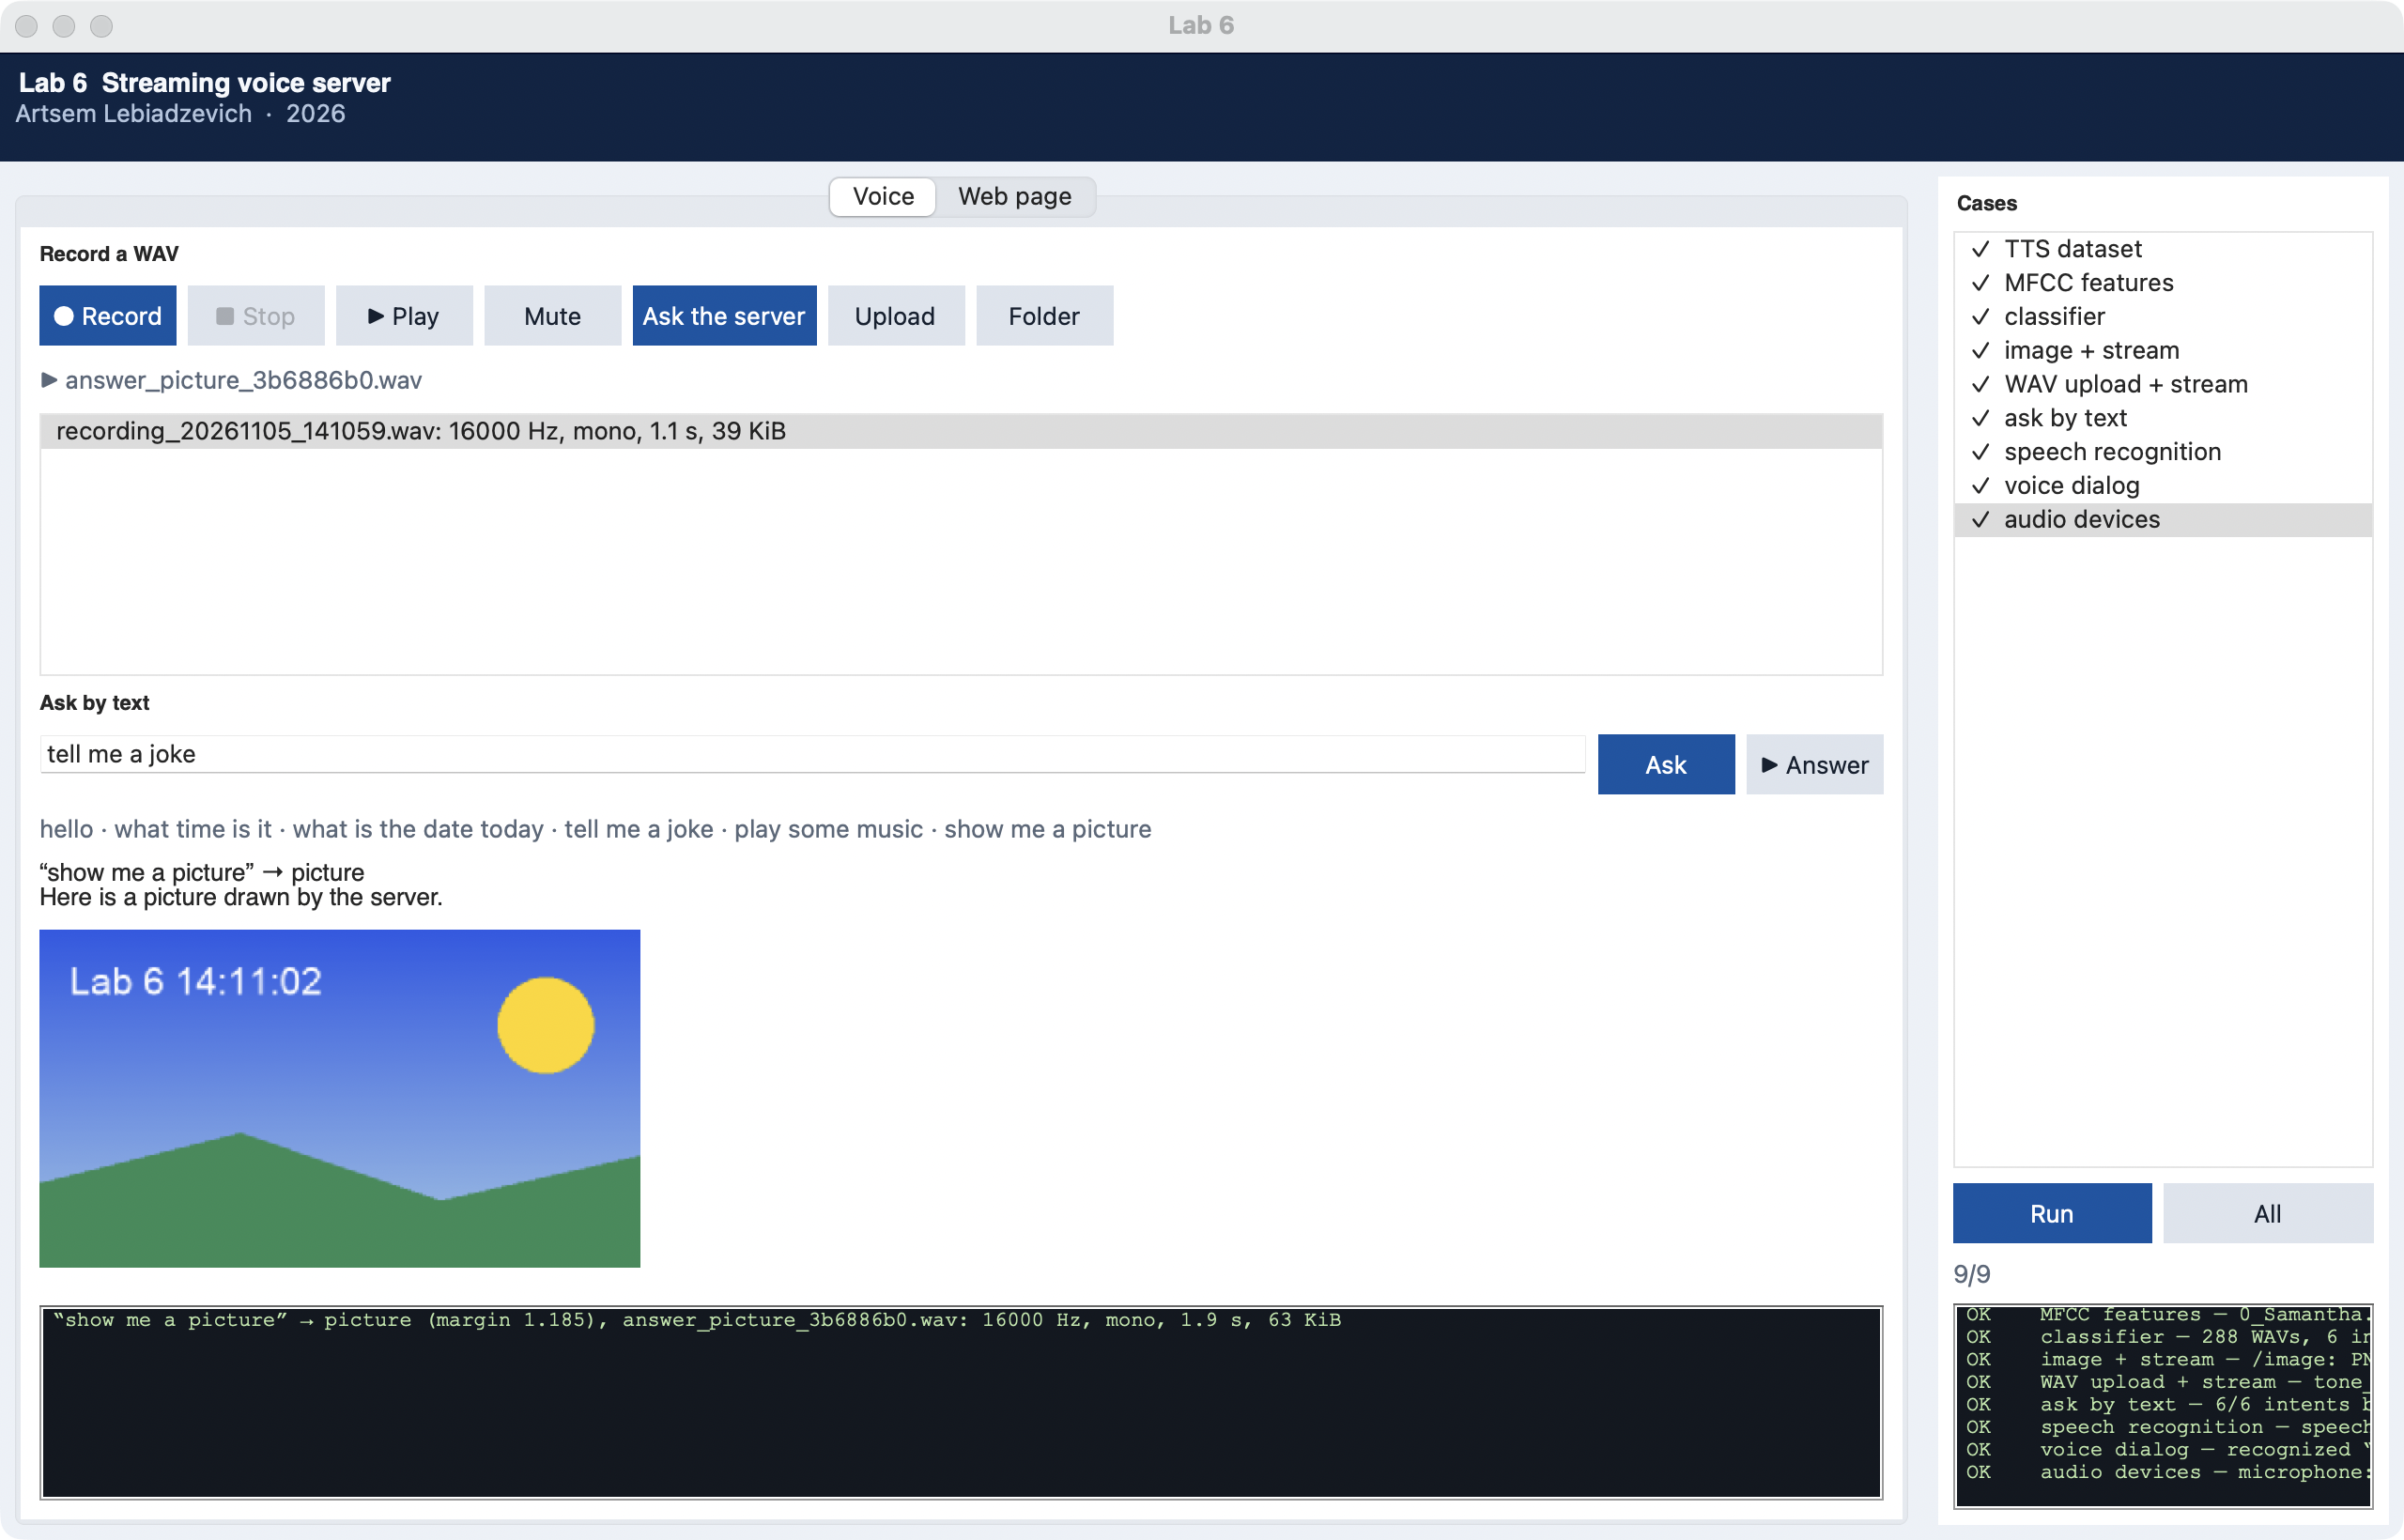
\includegraphics[width=0.95\textwidth]{../screenshots/lab6.png}
\caption{Окно лабораторной работы: запись, ответ сервера и список проверок}
\label{fig:window}
\end{figure}

На рисунке~\ref{fig:web} --- страница сервера во встроенном браузере: ответ на вопрос
<<play some music>> с проигрывателем, запись WAV, поток кадров часов и изображение.

\begin{figure}[H]
\centering
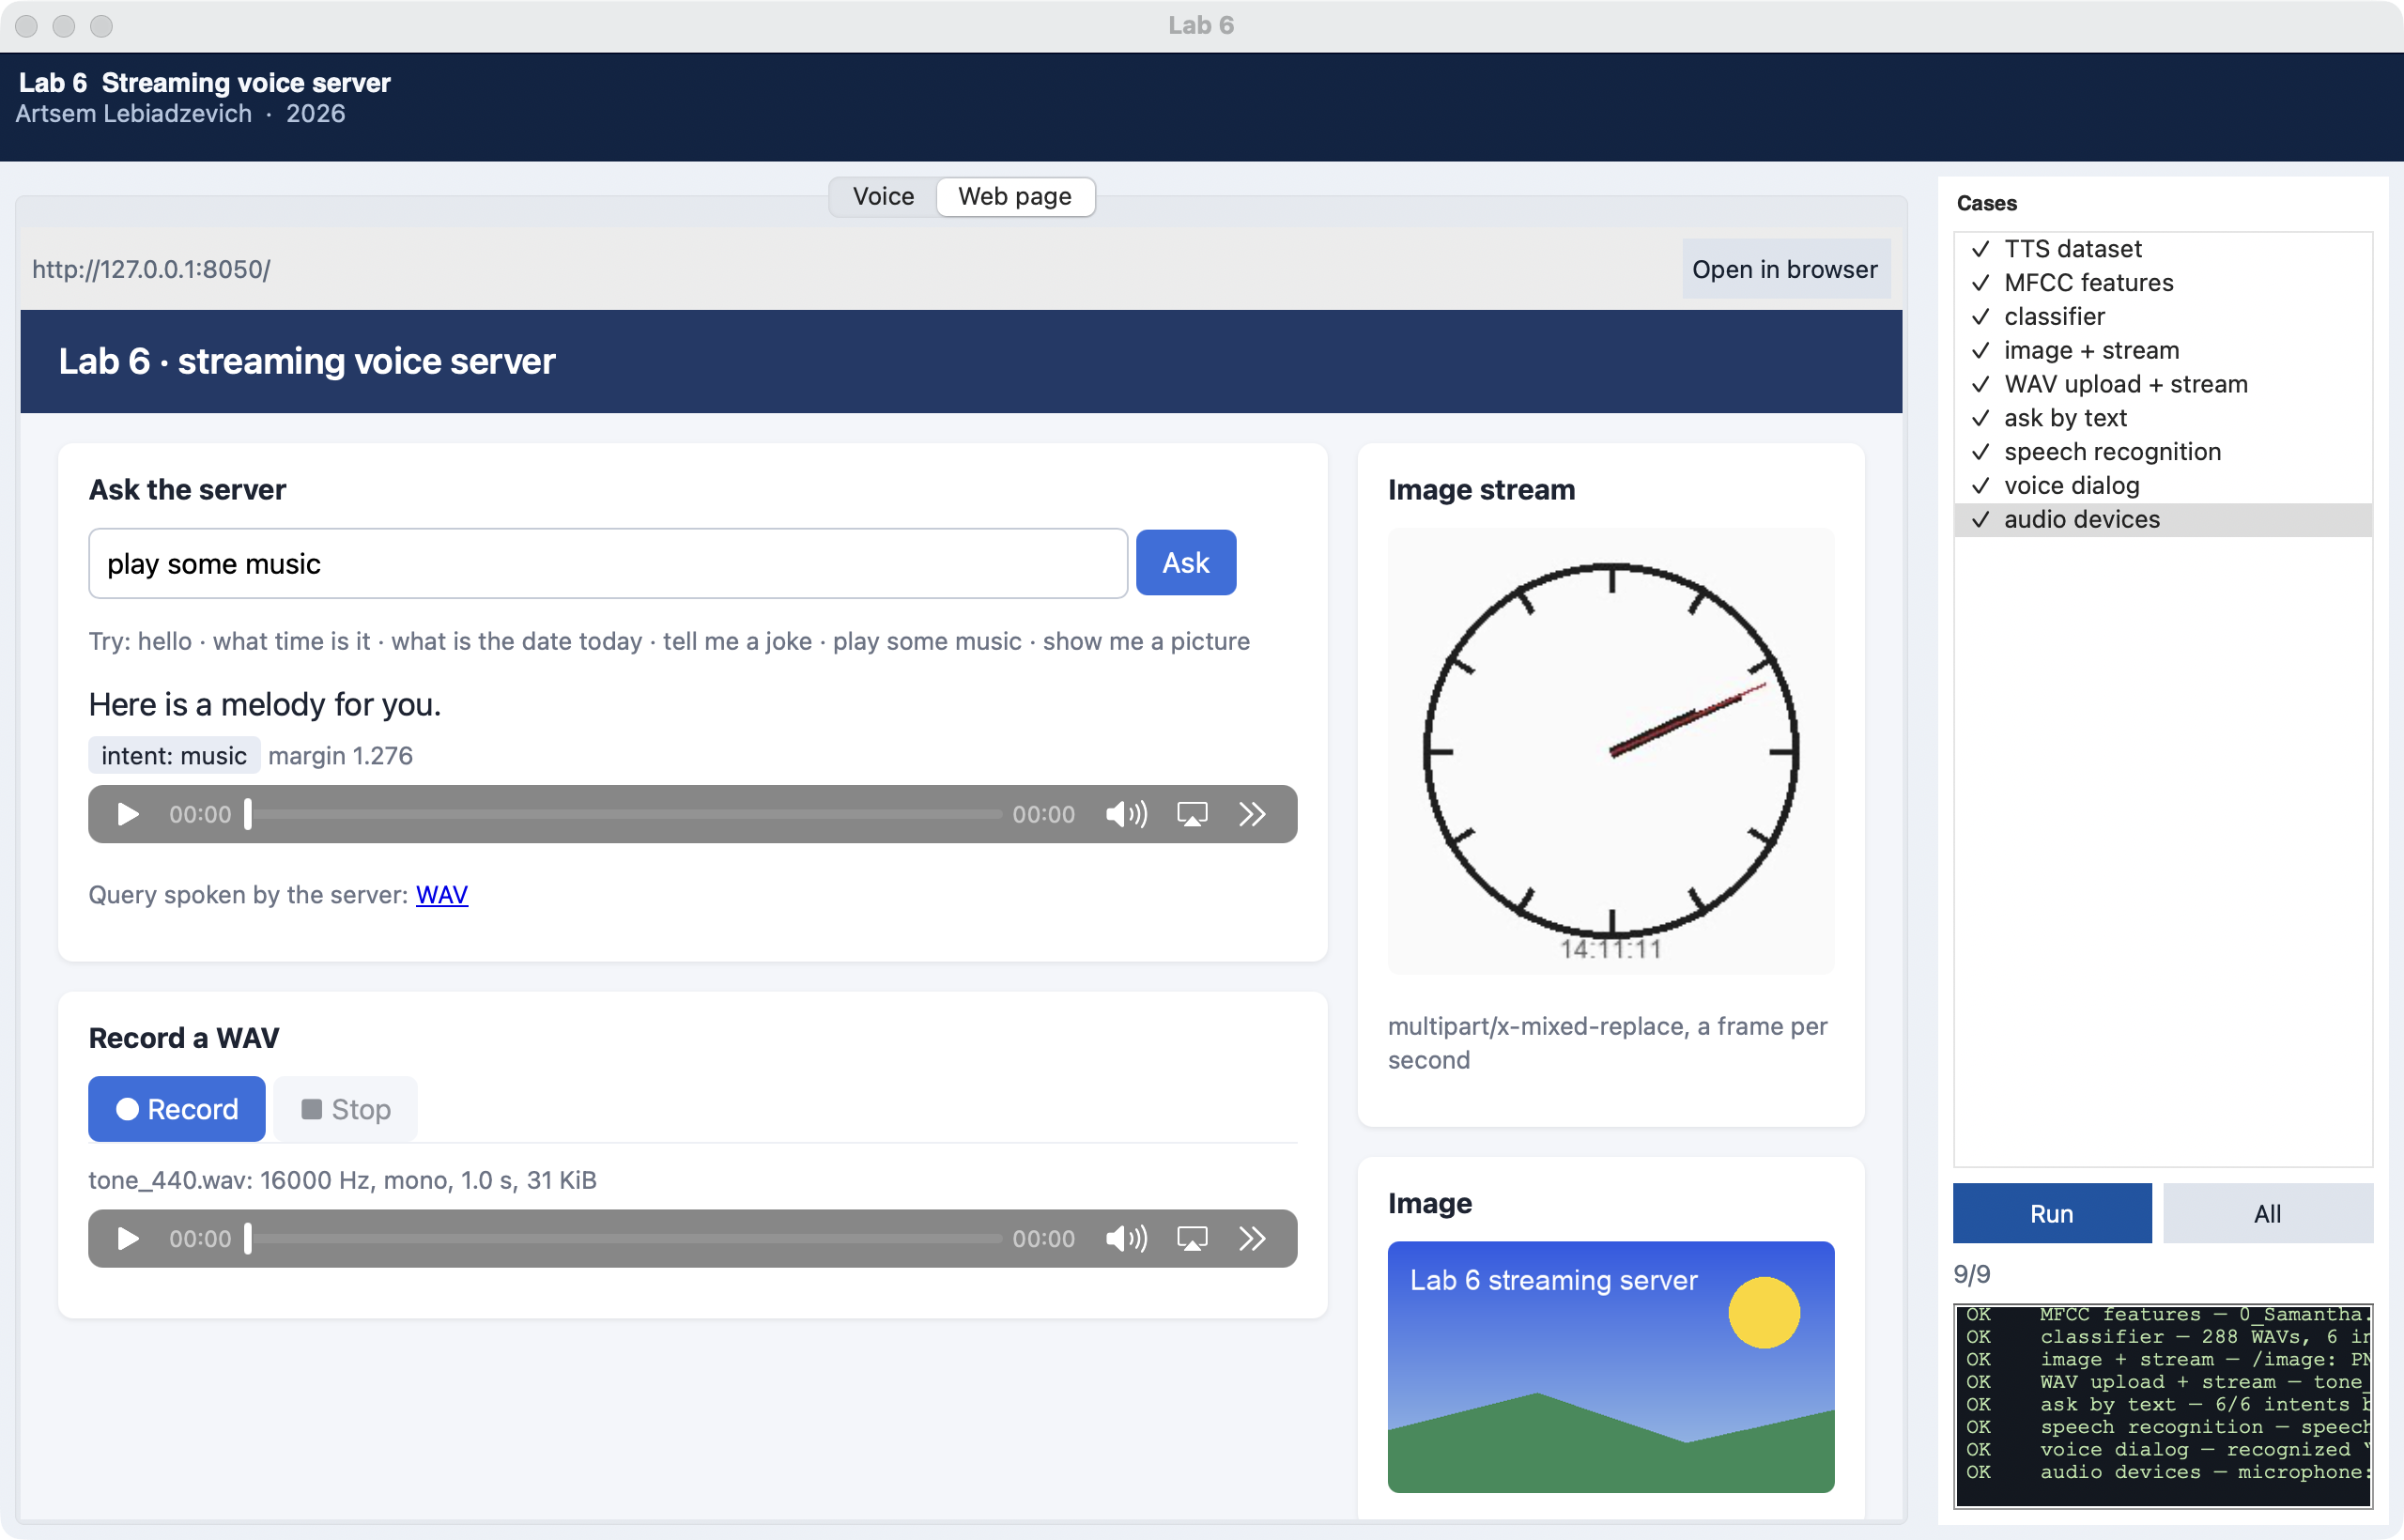
\includegraphics[width=0.95\textwidth]{../screenshots/lab6_web.png}
\caption{Страница потокового сервера}
\label{fig:web}
\end{figure}

Команда \texttt{python main.py -{}-lab 6} выполняет сценарии без окна; вывод приведён в
листинге~\ref{lst:cli}, содержание проверок --- в таблице~\ref{tab:results}.

\lstinputlisting[style=plain, breaklines=true, caption={Вывод программы}, label={lst:cli}]{listings/cli_output.txt}

\begin{table}[H]
\caption{Проверяемые сценарии}
\label{tab:results}
\centering
\small
\begin{tabularx}{\textwidth}{lL}
\toprule
Сценарий & Что проверяется \\
\midrule
TTS dataset & 288 WAV-файлов, ни один не короче 0,2~с \\
MFCC features & матрица MFCC из 13 столбцов, вектор из 78 признаков \\
classifier & точность на обучающих данных не ниже 90\,\%, на новых формулировках не
ниже 35\,\% \\
image + stream & \texttt{/image} отдаёт PNG; \texttt{/stream-image?frames=3} --- три
корректных кадра JPEG \\
WAV upload + stream & загруженный WAV возвращается без изменений; запрос
\texttt{Range: bytes=0-43} даёт ответ 206 с заголовком RIFF; запись есть в списке \\
ask by text & темы определяются по первой формулировке каждой, WAV ответа длиннее
0,5~с; ответ о времени содержит текущий час \\
speech recognition & речь <<tell me a joke>> распознаётся Google (без сети сценарий
пропускается) \\
voice dialog & полный цикл: WAV $\to$ текст $\to$ сервер $\to$ тема <<music>> $\to$
WAV ответа \\
audio devices & найдены микрофон и динамики \\
\bottomrule
\end{tabularx}
\end{table}

Автоматические тесты (\texttt{python -m unittest tests.test\_labs}) повторяют эти
проверки; все тесты проходят.

\section{Ответы на контрольные вопросы}

\textbf{1. Как web-сервер на Python возвращает изображение или звук?} Устанавливает
код 200 и заголовок \texttt{Content-Type} (\texttt{image/png}, \texttt{audio/wav}) и
записывает байты файла в \texttt{wfile}; браузер выводит их тегом \texttt{<img>} или
\texttt{<audio>}.

\textbf{2. Чем потоковая передача отличается от обычной?} Тело ответа передаётся
частями по мере чтения или создания данных. Для изображений используется
\texttt{multipart/x-mixed-replace}, для звука --- передача блоками и запросы
\texttt{Range}.

\textbf{3. Как записать и воспроизвести WAV на Python?} Входной поток PortAudio
(\texttt{sounddevice} или PyAudio) отдаёт блоки отсчётов, которые модуль
\texttt{wave} сохраняет в файл; для воспроизведения файл читается блоками и
записывается в выходной поток.

\textbf{4. Что такое MFCC?} Мел-кепстральные коэффициенты: спектр окна сигнала,
пропущенный через банк фильтров по шкале мел, прологарифмированный и преобразованный
ДКП. Они описывают огибающую спектра и служат признаками речи.

\textbf{5. Как построить классификатор WAV-файлов?} Подготовить размеченные файлы,
вычислить для каждого вектор признаков (MFCC и их статистики), обучить классификатор
(\texttt{SVC}) и проверять точность на файлах, не участвовавших в обучении.

\sectioncenter{Заключение}

В ходе лабораторной работы изучены потоковые web-серверы на \texttt{http.server},
запись и воспроизведение WAV-файлов, синтез и распознавание речи, признаки MFCC и
классификация звука. Создано приложение по схеме методических материалов: клиент
записывает голосовой запрос, распознаёт его и отправляет текст серверу; сервер
озвучивает текст, классификатором определяет тему и возвращает ответ в виде
WAV-файла, который воспроизводится у клиента. Сервер также передаёт изображение, поток
кадров и записи клиента.

Практический вывод: классификатор из пяти файлов методички проверялся на тех же файлах
и не показывал реальной точности. При честной проверке среднее MFCC узнаёт новую
формулировку в 40\,\% случаев; признаки, сохраняющие порядок звуков, и нелинейное ядро
повышают точность до 53\,\%, а надёжно распознаются фразы из обучающего набора. Для
браузера на WebKit сервер должен поддерживать запросы \texttt{Range}, иначе звук не
воспроизводится.

\sectioncenter{Список использованных источников}

\begin{enumerate}
\item Герман, О.~В. Потоковые web-серверы: лекция и лабораторная работа по дисциплине
<<Технологии компонентного программирования>> / О.~В.~Герман. --- Минск: БГУИР, 2024.
\item http.server --- HTTP servers [Электронный ресурс]. --- Режим доступа:
\url{https://docs.python.org/3/library/http.server.html}.
\item librosa: audio and music processing in Python [Электронный ресурс]. --- Режим
доступа: \url{https://librosa.org/doc/latest/}.
\item scikit-learn: Support Vector Machines [Электронный ресурс]. --- Режим доступа:
\url{https://scikit-learn.org/stable/modules/svm.html}.
\item SpeechRecognition [Электронный ресурс]. --- Режим доступа:
\url{https://pypi.org/project/SpeechRecognition/}.
\item python-sounddevice [Электронный ресурс]. --- Режим доступа:
\url{https://python-sounddevice.readthedocs.io/}.
\end{enumerate}

\end{document}
